\documentclass[10pt, twocolumn]{article}
\usepackage[utf8]{inputenc}
\usepackage[T1]{fontenc}
\usepackage[a4paper, margin=0.75in, columnsep=0.5cm]{geometry}
\usepackage{amsmath}
\usepackage{amsfonts}
\usepackage{amssymb}
\usepackage{mhchem}
\usepackage{graphicx}
\usepackage{caption}
\usepackage{booktabs}
\usepackage{array}
\usepackage{xcolor}
\usepackage{colortbl}
\usepackage{tikz}
\usetikzlibrary{arrows.meta, positioning}
\usepackage{eso-pic}
\usepackage{fancyhdr}
\usepackage{hyperref}
\usepackage{float}
\hypersetup{colorlinks=true, linkcolor=black, citecolor=black, urlcolor=blue}

% ---------------------------------------------------------
% Subtle page border on every page via eso-pic + TikZ
% ---------------------------------------------------------
\definecolor{bordergray}{RGB}{180,180,180}

\AddToShipoutPictureBG{%
  \begin{tikzpicture}[remember picture, overlay]
    \draw[color=bordergray, line width=0.5pt]
      ([xshift=14pt, yshift=-14pt]current page.north west)
      rectangle
      ([xshift=-14pt, yshift=14pt]current page.south east);
  \end{tikzpicture}%
}

% ---------------------------------------------------------
% Consistent header / footer via fancyhdr
% ---------------------------------------------------------
\pagestyle{fancy}
\fancyhf{}
\renewcommand{\headrulewidth}{0pt}
\renewcommand{\footrulewidth}{0pt}
\fancyfoot[C]{\small\thepage}

% Also apply to the first page (maketitle uses plain style)
\fancypagestyle{plain}{%
  \fancyhf{}
  \renewcommand{\headrulewidth}{0pt}
  \renewcommand{\footrulewidth}{0pt}
  \fancyfoot[C]{\small\thepage}
}

% ---------------------------------------------------------
\title{\textbf{SignFlow: Real-Time Assistive Captioning for Sign Language\\
Using 3D Landmark-Based Transformer Modeling}}
\author{}
\date{}

\begin{document}
\maketitle

\begin{abstract}
Sign language is the primary mode of communication for approximately 70 million deaf and hard-of-hearing individuals worldwide. Real-time automated interpretation remains an unsolved accessibility challenge: existing approaches are either unavailable in interactive contexts or limited to small vocabularies and specialised hardware. This paper presents \textbf{SignFlow}, an end-to-end pipeline classifying \textbf{58} ASL sign classes from live or on-screen video without depth sensors. The system extracts \textbf{92} three-dimensional skeletal landmarks per frame via MediaPipe Holistic, encodes them through body-part-specific multi-stream MLP embeddings, and classifies sign windows with \textbf{8} Transformer encoder blocks. Runtime input is variable-length: the client holds a 60-frame rolling buffer, the server downsamples to 40, and the model resamples to a fixed 64-frame tensor internally. A three-thread overlay decouples display, extraction, and inference, rendering an always-on-top PyQt5 caption layer without blocking the UI. Trained on $\approx$28,500 samples, SignFlow achieves \textbf{79.72\%} top-1 and \textbf{94.39\%} top-5 validation accuracy. Steady-state latency is in the low hundreds of milliseconds on a consumer GPU.
\end{abstract}

% =============================================================
\section*{1.~Introduction}
% =============================================================
Sign language recognition poses four interconnected challenges: (i) signs encode meaning in motion trajectories, requiring sequence-aware models; (ii) scaling to hundreds of classes is difficult under heavily imbalanced training data; (iii) real-world robustness demands tolerance to variation in hand size, speed, signing style, and occlusion; and (iv) the full pipeline must minimise user-perceived delay without blocking the UI on consumer hardware. Existing approaches fall short on at least one dimension: no real-time sign language equivalent of automatic speech recognition yet exists for consumer devices, human interpreters are costly to scale, and depth-camera systems remain impractical.

SignFlow addresses all four challenges simultaneously through a compact 3D landmark representation, a deep Transformer for temporal reasoning, comprehensive augmentation for cross-signer generalisation, and a decoupled three-thread overlay that keeps the display non-blocking at all times.

% =============================================================
\section*{2.~System Architecture}
% =============================================================

\subsection*{2.1~Pipeline Overview}

The end-to-end SignFlow pipeline proceeds through frame capture, landmark extraction, sequence normalisation, Transformer classification, and caption rendering. A core engineering contribution is its \textbf{zero-lag three-thread architecture}: display, landmark extraction, and model inference run in dedicated threads communicating via shared queues. The UI thread stays fully responsive; the extraction thread runs MediaPipe at $\approx$8\,FPS and dispatches HTTP requests to the Flask API every 150\,ms; the overlay thread consumes predictions and updates the caption without stalling capture.

\begin{figure}[h]
\centering
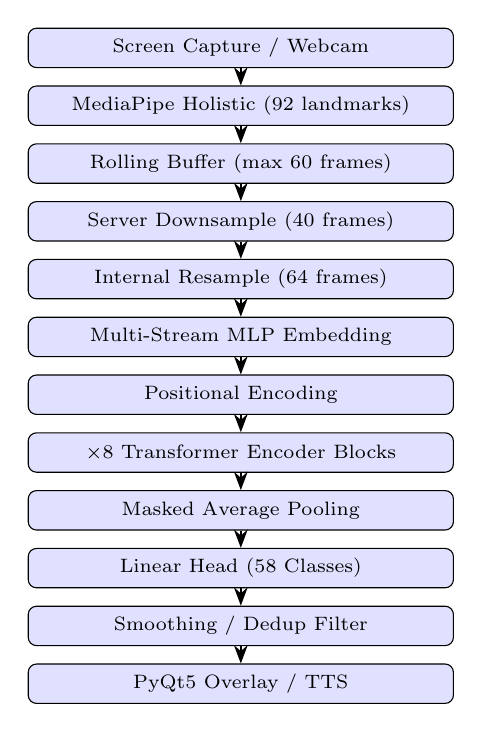
\begin{tikzpicture}[node distance=0.22cm]
  \tikzset{
    pnode/.style={rectangle, rounded corners=3pt, draw=black, fill=blue!12,
                  minimum width=5.4cm, minimum height=0.50cm,
                  text centered, align=center, font=\scriptsize},
    arr/.style={-Stealth, thick}
  }
  \node[pnode] (cap)  {Screen Capture / Webcam};
  \node[pnode, below=of cap]  (mp)   {MediaPipe Holistic (92 landmarks)};
  \node[pnode, below=of mp]   (buf)  {Rolling Buffer (max 60 frames)};
  \node[pnode, below=of buf]  (srv)  {Server Downsample (40 frames)};
  \node[pnode, below=of srv]  (res)  {Internal Resample (64 frames)};
  \node[pnode, below=of res]  (emb)  {Multi-Stream MLP Embedding};
  \node[pnode, below=of emb]  (pe)   {Positional Encoding};
  \node[pnode, below=of pe]   (tfm)  {$\times$8 Transformer Encoder Blocks};
  \node[pnode, below=of tfm]  (pool) {Masked Average Pooling};
  \node[pnode, below=of pool] (head) {Linear Head (58 Classes)};
  \node[pnode, below=of head] (filt) {Smoothing / Dedup Filter};
  \node[pnode, below=of filt] (disp) {PyQt5 Overlay / TTS};
  \foreach \a/\b in {cap/mp,mp/buf,buf/srv,srv/res,res/emb,
                     emb/pe,pe/tfm,tfm/pool,pool/head,head/filt,filt/disp}
    \draw[arr] (\a) -- (\b);
\end{tikzpicture}
\caption{Figure~1. End-to-end SignFlow pipeline: frame capture, landmark extraction,
sequence normalisation, Transformer classification, and caption rendering.}
\label{fig:pipeline}
\end{figure}

\subsection*{2.2~Module Descriptions}

\subsubsection*{2.2.1~Input Capture and Landmark Extraction}
SignFlow supports \emph{screen-capture mode}, processing any on-screen application without the signer being co-located, and \emph{webcam mode} for a live camera feed. MediaPipe Holistic~\cite{mediapipe} processes each frame via a 468-point face mesh, 21-point per-hand tracking, and 33-point pose model. A curated subset of \textbf{92} landmarks is retained (Table~\ref{tab:landmarks}); occluded landmarks are zero-filled.

\begin{table}[h]
\centering
\caption{Table~1. Landmark composition per video frame.}
\label{tab:landmarks}
\setlength{\tabcolsep}{3pt}
\small
\begin{tabular}{|l|c|c|p{2.2cm}|}
\hline
\textbf{Region} & \textbf{Pts} & \textbf{Dim} & \textbf{Description} \\
\hline
Lips (outer + inner) & 40 & 120 & Mouth shape \\
\hline
Left Hand  & 21 & 63 & Wrist + joints \\
\hline
Right Hand & 21 & 63 & Same as left \\
\hline
Upper Body Pose & 10 & 30 & Shoulders, elbows, etc. \\
\hline
\textbf{Total} & \textbf{92} & \textbf{276} & $92\times3$ floats/frame \\
\hline
\end{tabular}
\end{table}

\subsubsection*{2.2.2~Buffer, Smoothing and Caption Logic}
The client starts predicting after \textbf{5 frames}, maintaining a rolling buffer of up to \textbf{60 frames}; the server downsamples to 40 and the model resamples internally to a fixed 64-frame tensor. The buffer resets on a hand-loss timeout, segmenting utterances automatically. Before display, predictions pass through: (i)~duplicate suppression; (ii)~hold-and-confirm committing a sign after 8 consecutive matching cycles; (iii)~exponential smoothing ($p_t = 0.70\,p_\text{new}+0.30\,p_{t-1}$); and (iv)~automatic buffer reset on prolonged hand disappearance.

\subsubsection*{2.2.3~Backend and Overlay}
A Flask REST server loads the PyTorch checkpoint at startup, accepts landmark sequences over HTTP, and returns the top-1 prediction with top-5 confidence scores. It supports a local Ollama mode and a cloud Gemini mode, and is deployable as a Windows-native service or via a Render manifest. In the primary path, duplicate-suppressed tokens render directly in a translucent always-on-top PyQt5 window; an optional TTS module provides audio output.

% =============================================================
\section*{3.~Methodology}
% =============================================================

\subsection*{3.1~Input Representation and Multi-Stream Embedding}
Each sequence is resampled to 64 frames, yielding a tensor of shape $(\text{Batch},\,64,\,92,\,3)$. The four body-part streams are embedded independently:
\[
  \mathbf{h}_i = \operatorname{LayerNorm}\!\bigl(W_2\,\operatorname{GELU}(W_1\mathbf{x}_i+b_1)+b_2\bigr)
\]
and fused via learned softmax weights so the model dynamically up-weights the most informative body part per sign:
\[
  \mathbf{w} = \operatorname{softmax}\!\bigl([w_\text{lips},\,w_\text{LH},\,w_\text{RH},\,w_\text{pose}]\bigr)
\]
\[
  \mathbf{e}_\text{fused} = \textstyle\sum_i w_i\,\mathbf{e}_i
\]

\subsection*{3.2~Transformer Architecture}

Each of the 8 encoder blocks applies pre-norm MHA then MLP:
\[
  \mathbf{x} \leftarrow \mathbf{x}+\operatorname{MHA}(\operatorname{LN}(\mathbf{x}))
\]
\[
  \mathbf{x} \leftarrow \mathbf{x}+\operatorname{MLP}(\operatorname{LN}(\mathbf{x}))
\]
A key-padding mask suppresses zero-padded frames. Masked average pooling collapses the temporal axis to a single vector, projected by a linear head to 58 classes. Table~\ref{tab:transformer} lists the full configuration.

\begin{figure}[h]
\centering
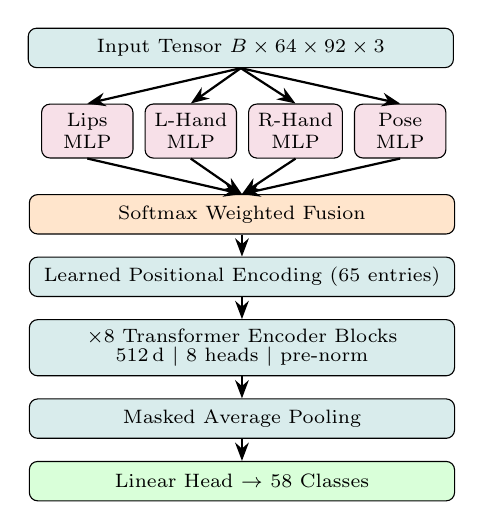
\begin{tikzpicture}[node distance=0.28cm and 0.14cm]
  \tikzset{
    mnode/.style={rectangle, rounded corners=3pt, draw=black, fill=teal!15,
                  minimum width=5.4cm, minimum height=0.50cm,
                  text centered, align=center, font=\scriptsize},
    snode/.style={rectangle, rounded corners=3pt, draw=black, fill=purple!12,
                  minimum width=1.16cm, minimum height=0.65cm,
                  text centered, align=center, font=\scriptsize},
    fnode/.style={rectangle, rounded corners=3pt, draw=black, fill=orange!20,
                  minimum width=5.4cm, minimum height=0.50cm,
                  text centered, align=center, font=\scriptsize},
    onode/.style={rectangle, rounded corners=3pt, draw=black, fill=green!15,
                  minimum width=5.4cm, minimum height=0.50cm,
                  text centered, align=center, font=\scriptsize},
    arr/.style={-Stealth, thick}
  }
  % Input
  \node[mnode] (inp) {Input Tensor $B \times 64 \times 92 \times 3$};
  % Four parallel streams — centred under inp
  \node[snode, below=0.45cm of inp, xshift=-1.95cm] (lips) {Lips\\MLP};
  \node[snode, right=0.14cm of lips]                (lh)   {L-Hand\\MLP};
  \node[snode, right=0.14cm of lh]                  (rh)   {R-Hand\\MLP};
  \node[snode, right=0.14cm of rh]                  (pose) {Pose\\MLP};
  % Fusion and remainder
  \node[fnode, below=0.45cm of lh, xshift=0.65cm]   (fuse) {Softmax Weighted Fusion};
  \node[mnode, below=0.28cm of fuse] (pe)   {Learned Positional Encoding (65 entries)};
  \node[mnode, below=0.28cm of pe]   (tfm)  {$\times$8 Transformer Encoder Blocks\\[-1pt]
                                              512\,d $|$ 8 heads $|$ pre-norm};
  \node[mnode, below=0.28cm of tfm]  (pool) {Masked Average Pooling};
  \node[onode, below=0.28cm of pool] (out)  {Linear Head $\rightarrow$ 58 Classes};
  % Arrows from input to streams
  \foreach \s in {lips,lh,rh,pose}
    \draw[arr] (inp.south) -- (\s.north);
  % Arrows from streams to fusion
  \foreach \s in {lips,lh,rh,pose}
    \draw[arr] (\s.south) -- (fuse.north);
  % Remaining vertical arrows
  \foreach \a/\b in {fuse/pe,pe/tfm,tfm/pool,pool/out}
    \draw[arr] (\a) -- (\b);
\end{tikzpicture}
\caption{Figure~2. Model architecture: four anatomical streams embed independently,
fuse via softmax weighting, then pass through the Transformer stack.
Masked average pooling yields one sign prediction per window.}
\label{fig:model}
\end{figure}

\begin{table}[h]
\centering
\caption{Table~2. Transformer encoder configuration.}
\label{tab:transformer}
\small
\begin{tabular}{|l|l|}
\hline
\textbf{Hyperparameter} & \textbf{Value} \\
\hline
Encoder blocks / Hidden dim & 8 / 512 \\
\hline
Attention heads / Head dim & 8 / 64 \\
\hline
MLP ratio & $4\times$ $(512{\to}2048{\to}512)$ \\
\hline
Attn / MLP / Embed dropout & 0.10 / 0.20 / 0.10 \\
\hline
Total trainable parameters & 26,642,161 \\
\hline
\end{tabular}
\end{table}

\subsection*{3.3~Training Data, Augmentation, and Optimisation}
Signs were curated from three sources and filtered to the shared 58-class vocabulary (Tables~\ref{tab:dataset} and~\ref{tab:vocab}).

\begin{table}[h]
\centering
\caption{Table~3. Dataset composition (80/20 train-val split).}
\label{tab:dataset}
\small
\setlength{\tabcolsep}{3pt}
\begin{tabular}{|l|c|c|p{1.8cm}|}
\hline
\textbf{Source} & \textbf{Signs} & \textbf{Samples} & \textbf{Notes} \\
\hline
WLASL~\cite{wlasl}    & 58 & $\approx$25,000 & Matching signs \\
\hline
MS-ASL~\cite{msasl}   & 58 & $\approx$2,000  & Matching signs \\
\hline
Custom (YouTube)       & 13 & $\approx$1,500  & Self-collected \\
\hline
\textbf{Total}         & \textbf{58} & $\approx$\textbf{28,500} & Combined \\
\hline
\end{tabular}
\end{table}

Nine augmentation strategies improve robustness: temporal crop, speed perturbation, horizontal flip with handedness swap, spatial jitter ($\sigma=0.005$), random scale and in-plane rotation, and per-stream dropout (frame, lip, hand, pose independently). Mixup~\cite{mixup} ($\alpha=0.2$) is applied at batch level. Training uses AdamW ($\text{lr}=5\times10^{-5}$, cosine annealing, FP16 mixed precision); SWA~\cite{swa} activates after epoch~120.

\subsection*{3.4~Token-to-English Conversion}
In the local path, accumulated sign tokens are passed to an LLM with a prompt requesting reconstruction of grammatically correct English sentences, correction of recognition errors, and preservation of the original intent. This bridges the gap between ASL grammar (topic-comment order, spatial inflection) and English syntax. In the deployed remote overlay path this step is instrumented in logging but not yet wired into the live loop.

% =============================================================
\section*{4.~Results and Performance}
% =============================================================

\subsection*{4.1~Training Progression}
Validation accuracy surpasses 78\% by epoch 4 and peaks at \textbf{79.72\%} at epoch 9 (Table~\ref{tab:epochs}). The $\approx$14-point gap between training (93.03\%) and validation accuracy arises from classification-head re-initialisation during Phase-2 transfer, class imbalance, and intrinsic similarity between visually adjacent signs. The top-5 accuracy of 94.39\%---the correct sign among the five most confident predictions in the vast majority of cases---is directly useful for soft-matching and beam-search decoding in continuous captioning.

\begin{table}[h]
\centering
\caption{Table~5. Validation accuracy across key epochs. \colorbox{yellow!40}{Shaded: best checkpoint.}}
\label{tab:epochs}
\small
\begin{tabular}{|c|c|c|c|}
\hline
\textbf{Epoch} & \textbf{Train} & \textbf{Top-1} & \textbf{Top-5} \\
\hline
1  & 13.10\% & 35.65\% & 57.74\% \\
2  & 75.76\% & 70.10\% & 89.57\% \\
3  & 89.11\% & 76.08\% & 92.90\% \\
4  & 91.61\% & 78.27\% & 93.81\% \\
7  & 92.73\% & 79.36\% & 94.25\% \\
\rowcolor{yellow!40}
9  & 93.03\% & \textbf{79.72\%} & \textbf{94.39\%} \\
28 & 93.95\% & 76.57\% & 93.35\% \\
\hline
\end{tabular}
\end{table}

\subsection*{4.2~System Performance and Latency}
Table~\ref{tab:perf} summarises system metrics. Time-to-first-prediction is $\gtrsim 0.8$\,s (five frames at $\approx$8\,FPS); steady-state user-visible delay is in the low hundreds of milliseconds. Common signs (``help'', ``thank you'', ``stop'', ``I love you'') were reliably recognised under standard indoor lighting. Duplicate suppression eliminated caption flicker; the 8-cycle hold-and-confirm threshold reduced false commits from transient noise. The most frequent failure modes were missing face/lip landmarks on certain webcam angles and ambiguous dual-hand handedness assignment by MediaPipe. CPU-only inference degrades throughput significantly, confirming GPU dependency for real-time operation.

\begin{table}[h]
\centering
\caption{Table~6. SignFlow system performance metrics.}
\label{tab:perf}
\small
\begin{tabular}{|p{2.8cm}|p{2.6cm}|}
\hline
\textbf{Metric} & \textbf{Value} \\
\hline
Val.\ Top-1 / Top-5 & 79.72\% / 94.39\% \\
\hline
Sign vocabulary & 58 classes \\
\hline
Trainable parameters & 26,642,161 \\
\hline
Internal seq.\ length & 64 frames \\
\hline
Client / Server buffer & 60 / 40 frames \\
\hline
Extraction / Pred.\ rate & $\approx$8\,FPS / 150\,ms \\
\hline
Time-to-first pred. & $\gtrsim 0.8$\,s \\
\hline
Steady-state delay & Low hundreds of ms \\
\hline
Hardware & NVIDIA RTX 3070\,Ti \\
\hline
\end{tabular}
\end{table}

% =============================================================
\section*{5.~Applications}
% =============================================================
SignFlow operates as a general-purpose accessibility layer: everyday conversations between a signer and a hearing person without a third-party interpreter; video conferencing (Zoom, Google Meet, Teams) by positioning the overlay over any conferencing window; education, giving deaf students access to signing instructors without recurring interpreter costs; and public-sector kiosks (healthcare, government), where Ollama mode runs entirely locally to preserve privacy.

% =============================================================
\section*{6.~Limitations and Future Work}
% =============================================================
\textbf{Limitations:} (i) the 58-sign vocabulary covers daily interaction but falls far short of full ASL; (ii) the fixed 64-frame window cannot model co-articulated continuous signing without CTC or dynamic segmentation; (iii) the LLM grammar rewrite is not yet active in the primary path; (iv) landmark extraction degrades under poor lighting, extreme angles, and heavy occlusion; (v) real-time throughput requires a discrete GPU; (vi) no explicit signer-independence training.

\textbf{Planned work:} wiring LLM rewrite into the live loop; scaling to 2,000+ signs via few-shot learning and pose-based synthesis; replacing the fixed-window classifier with a CTC-based continuous decoder; extending to ISL, BSL, and LSF via cross-lingual transfer; and knowledge distillation for edge deployment.

% =============================================================
\section*{7.~Conclusion}
% =============================================================

SignFlow is a real-time ASL recognition and captioning system that bridges communication between deaf and hearing users. It uses a multi-stream 3D Landmark Transformer to process lip, hand, and pose data, classifying signs through eight encoder blocks. With a zero-lag three-thread architecture, it ensures smooth, non-blocking performance. Trained on $\approx$28{,}500 samples across 58 classes, it achieves \textbf{79.72\%} top-1 and \textbf{94.39\%} top-5 accuracy with low-latency performance on consumer GPUs.

% =============================================================
% Full-width vocabulary table (two-column spanning)
% =============================================================
% \onecolumn
\vspace{30pt}
\begin{table*}[!t]
\centering
\caption{Table~4. Complete SignFlow vocabulary (58 classes, indices 0--57).}
\label{tab:vocab}

\renewcommand{\arraystretch}{1.3} % increase row height
\setlength{\tabcolsep}{6pt}       % increase column spacing

\resizebox{\textwidth}{!}{%
\begin{tabular}{|c|l|c|l|c|l|c|l|}
\hline
\textbf{ID} & \textbf{Sign} & \textbf{ID} & \textbf{Sign} & \textbf{ID} & \textbf{Sign} & \textbf{ID} & \textbf{Sign}\\
\hline
0  & hello             & 15 & stop      & 30 & sad       & 45 & time    \\
1  & thank you         & 16 & want      & 31 & hungry    & 46 & dad     \\
2  & help              & 17 & love      & 32 & hot       & 47 & mom     \\
3  & sorry             & 18 & need      & 33 & old       & 48 & brother \\
4  & please            & 19 & eat       & 34 & sick      & 49 & man     \\
5  & yes               & 20 & drink     & 35 & thirsty   & 50 & boy     \\
6  & no                & 21 & make      & 36 & mad       & 51 & grandma \\
7  & what is your name & 22 & see       & 37 & cute      & 52 & grandpa \\
8  & I love you        & 23 & talk      & 38 & better    & 53 & water   \\
9  & i                 & 24 & wake      & 39 & fine      & 54 & food    \\
10 & he / she / it     & 25 & open      & 40 & day       & 55 & milk    \\
11 & what              & 26 & cry       & 41 & night     & 56 & apple   \\
12 & how               & 27 & stay      & 42 & yesterday & 57 & home    \\
13 & when              & 28 & buy       & 43 & tomorrow  &    &         \\
14 & where             & 29 & cook      & 44 & later     &    &         \\
\hline
\end{tabular}
}
\end{table*}

\onecolumn
\newpage
\begin{thebibliography}{15}

\bibitem{mediapipe}
Zhang, F.\ et al.\ (2020). MediaPipe Holistic: Simultaneous Face, Hand, and Pose Prediction on Device. \textit{Google Research Technical Report}.

\bibitem{wlasl}
Li, D., Rodriguez, C., Yu, X., and Li, H.\ (2020). Word-Level Deep Sign Language Recognition from Video: A New Large-Scale Dataset and Methods Comparison. In \textit{Proc.\ IEEE WACV}.

\bibitem{msasl}
Joze, H.\,R.\,V.\ and Koller, O.\ (2019). MS-ASL: A Large-Scale Data Set and Benchmark for Understanding American Sign Language. \textit{arXiv:1812.01053}.

\bibitem{attention}
Vaswani, A.\ et al.\ (2017). Attention Is All You Need. In \textit{Proc.\ NeurIPS}, vol.~30.

\bibitem{vit}
Dosovitskiy, A.\ et al.\ (2021). An Image Is Worth $16{\times}16$ Words: Transformers for Image Recognition at Scale. In \textit{Proc.\ ICLR}.

\bibitem{swa}
Izmailov, P.\ et al.\ (2018). Averaging Weights Leads to Wider Optima and Better Generalization. In \textit{Proc.\ UAI}.

\bibitem{mixup}
Zhang, H.\ et al.\ (2018). mixup: Beyond Empirical Risk Minimization. In \textit{Proc.\ ICLR}.

\bibitem{mediapipe2}
Lugaresi, C.\ et al.\ (2019). MediaPipe: A Framework for Building Perception Pipelines. \textit{arXiv:1906.08172}.

\bibitem{camgoz2020}
Camgoz, N.\,C., Koller, O., Hadfield, S., and Bowden, R.\ (2020). Sign Language Transformers: Joint End-to-End Sign Language Recognition and Translation. In \textit{Proc.\ IEEE/CVF CVPR}, pp.~10023--10033.

\bibitem{openpose}
Cao, Z., Simon, T., Wei, S.-E., and Sheikh, Y.\ (2017). Realtime Multi-Person 2D Pose Estimation Using Part Affinity Fields. In \textit{Proc.\ IEEE CVPR}, pp.~7291--7299.

\bibitem{samslr}
Jiang, S., Sun, B., Wang, L., Bai, Y., Li, K., and Fu, Y.\ (2021). Skeleton Aware Multi-Modal Sign Language Recognition. In \textit{Proc.\ IEEE/CVF CVPRW}, pp.~3408--3418.

\bibitem{ctc}
Graves, A., Fern\'{a}ndez, S., Gomez, F., and Schmidhuber, J.\ (2006). Connectionist Temporal Classification. In \textit{Proc.\ ICML}, pp.~369--376.

\bibitem{zhou2022}
Zhou, H., Zhou, W., Zhou, Y., and Li, H.\ (2022). Spatial-Temporal Multi-Cue Network for Sign Language Recognition and Translation. \textit{IEEE Trans.\ Multimedia}, 24, pp.~768--779.

\bibitem{koller2020}
Koller, O.\ (2020). Quantitative Survey of the State of the Art in Sign Language Recognition. \textit{arXiv:2008.09918}.

\bibitem{bohacek2022}
Boh\'{a}\v{c}ek, M.\ and Hr\'{u}z, M.\ (2022). Sign Pose-Based Transformer for Word-Level Sign Language Recognition. In \textit{Proc.\ IEEE/CVF WACVW}, pp.~3429--3438.

\end{thebibliography}

\end{document}
